
\subsection{Single Lepton Top MC Modelling Validation from CR2}
\label{sec:cr2}

IS THIS GOING TO BE DONE WITH A BVETO OR NOT.  IF SO, IS IT GOING TO
BE CSVL OR CSVM?  NEED TO DISCUSS THIS.

The \mt\ tail for single-lepton top events (\ttsl\ and single top) is dominated by jet resolution effects. The \W\ cannot be far off-shell because $\mW < \mtop$.
The modeling of the \mt\ tail from jet resolution effects is studied using \zjets\ data and MC samples. 
\Z\ events are selection by requiring 2 good leptons (satisfying ID and isolation requirements) and requiring the \mll\ to be in the range $81-101$ GeV. 
The negative lepton is treated as a neutrino and so is added to the MET: \met\ $\rightarrow$ \pt(\Lepm) + \met, 
and the \mt\ is recalculated with the positive lepton \mt(\Lepp, \met).
The resulting ``pseudo-\mt'' is dominated by jet resolution effects, since no off-shell 
\Z\ production enters the sample due to the \mll\ requirement.
This section describes how well the MC predicts the tail of ``pseudo-\mt''. 

The underlying distributions are shown in Fig.~\ref{fig:cr2met}
and~\ref{fig:cr2mtrest}.  The comparison of data and MC event counts 
is shown in Table~\ref{tab:cr2yields}.  From this table we extract
the data to MC scale factors $SFR^{e}_{top}$ and  $SFR^{\mu}_{top}$. 


\begin{table}[!h]
\begin{center}
\begin{tabular}{l||c|c||c|c|c|c}
\hline
Sample              & CR2PRESEL0 &CR2PRESEL1 & CR2A & CR2B & CR2C & CR2D \\
\hline
\hline
DY MC 		  & $35 \pm 2$ & $30 \pm 2$ & $18 \pm 2$ & $32 \pm 3$ & $12 \pm 2$ & $5 \pm 1$ \\
Data - non-DY MC 	  & $65 \pm 9$ & $50 \pm 8$ & $36 \pm 6$ & $49 \pm 7$ & $25 \pm 5$ & $14 \pm 4$ \\
\hline
Data/MC SF 	  & $1.88 \pm 0.29$ & $1.68 \pm 0.30$ & $1.94 \pm 0.40$ & $1.54 \pm 0.29$ & $2.12 \pm 0.58$ & $2.96 \pm 1.22$ \\
\hline
\end{tabular}
\caption{ Yields in \mt\ tail comparing the MC prediction (after
  applying SFs) to data. CR2PRESEL refers to a sample with $\met>50$
  GeV and $\mt>150$ GeV.
  The uncertainties are statistical only.  NEED TO ADD THE SYMBOLS
  DEFINED IN THE TEXT FOR THESE SCALE FACTORS.  IS THIS GOING TO BE
  DONE SEPARATELY FOR MUONS AND ELECTRONS???
\label{tab:cr2yields}}
\end{center}
\end{table}

\begin{figure}[hbt]
  \begin{center}
	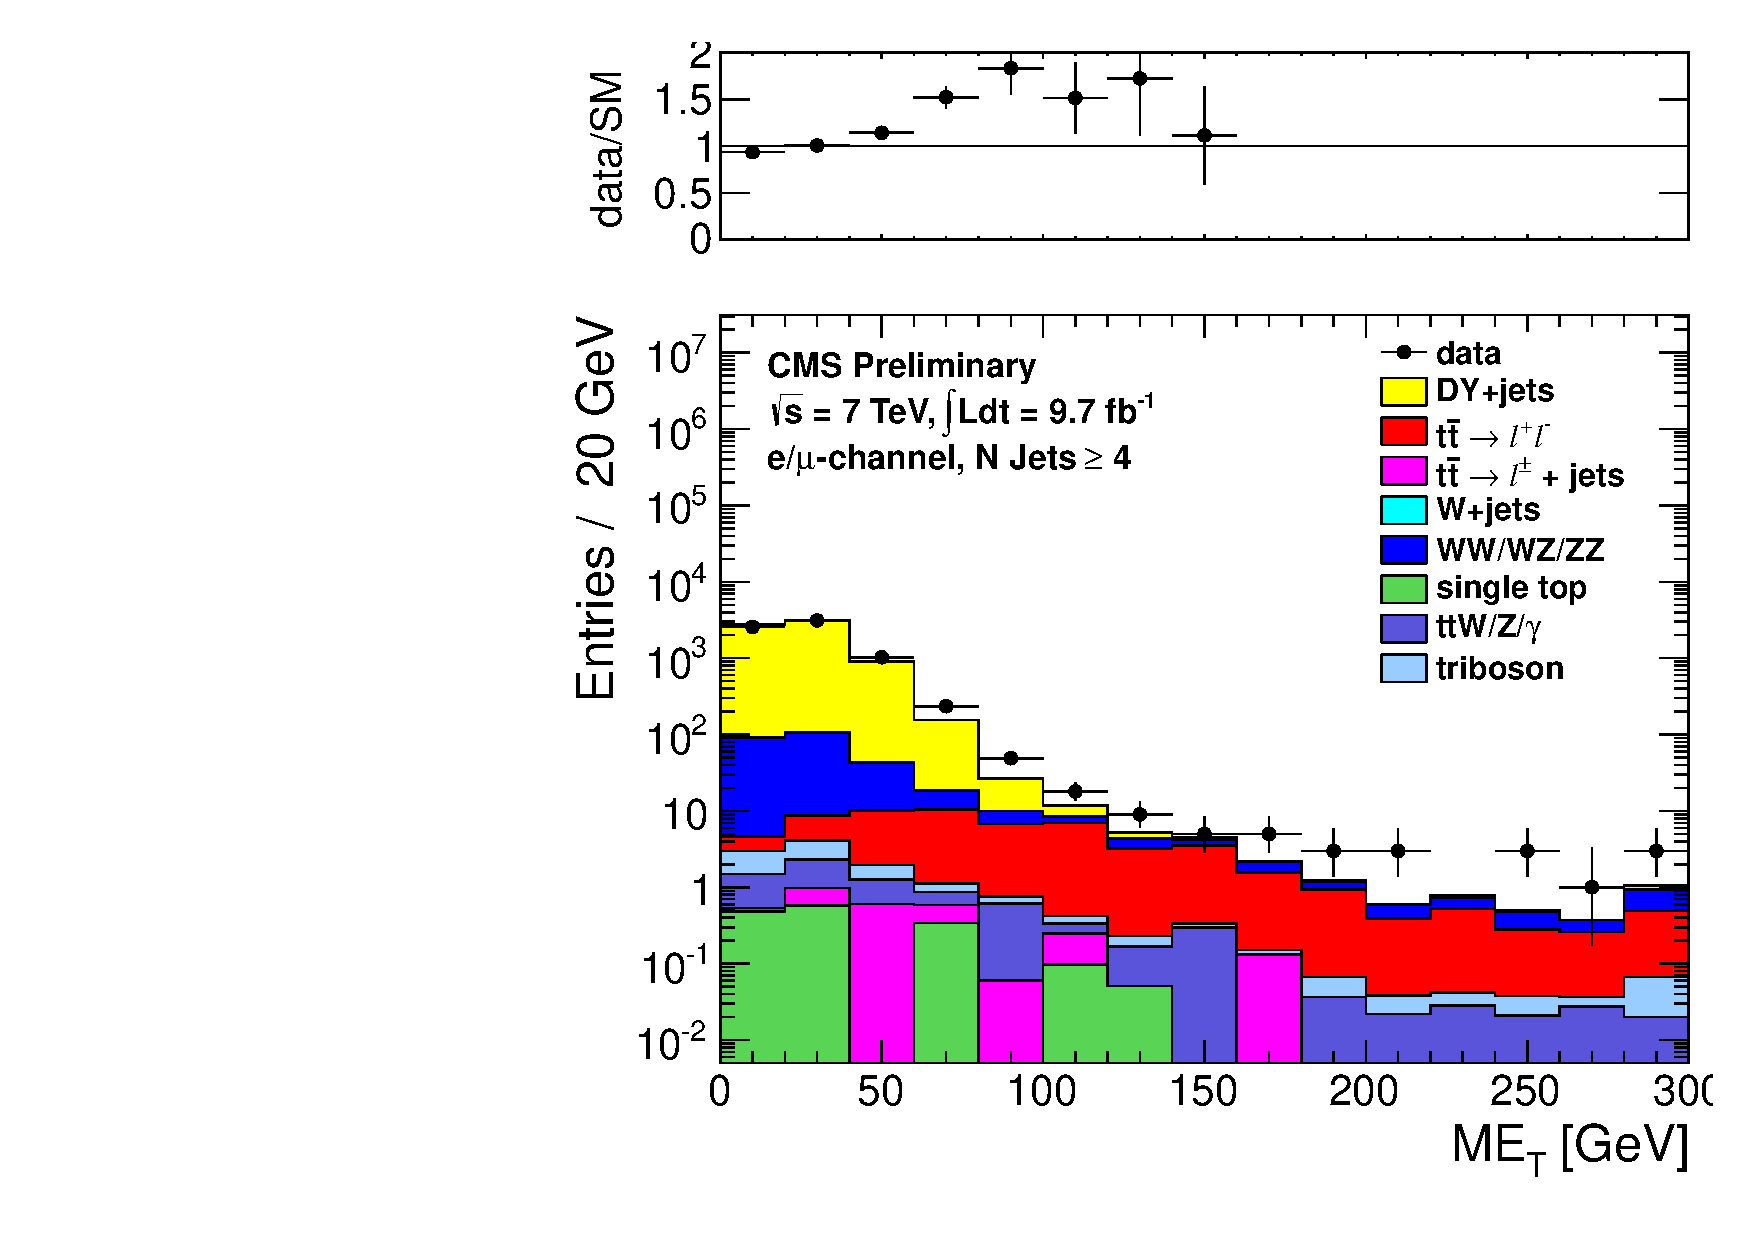
\includegraphics[width=0.5\linewidth]{plots/CR2plots/met_scaled_nj4_emucomb.pdf}%
	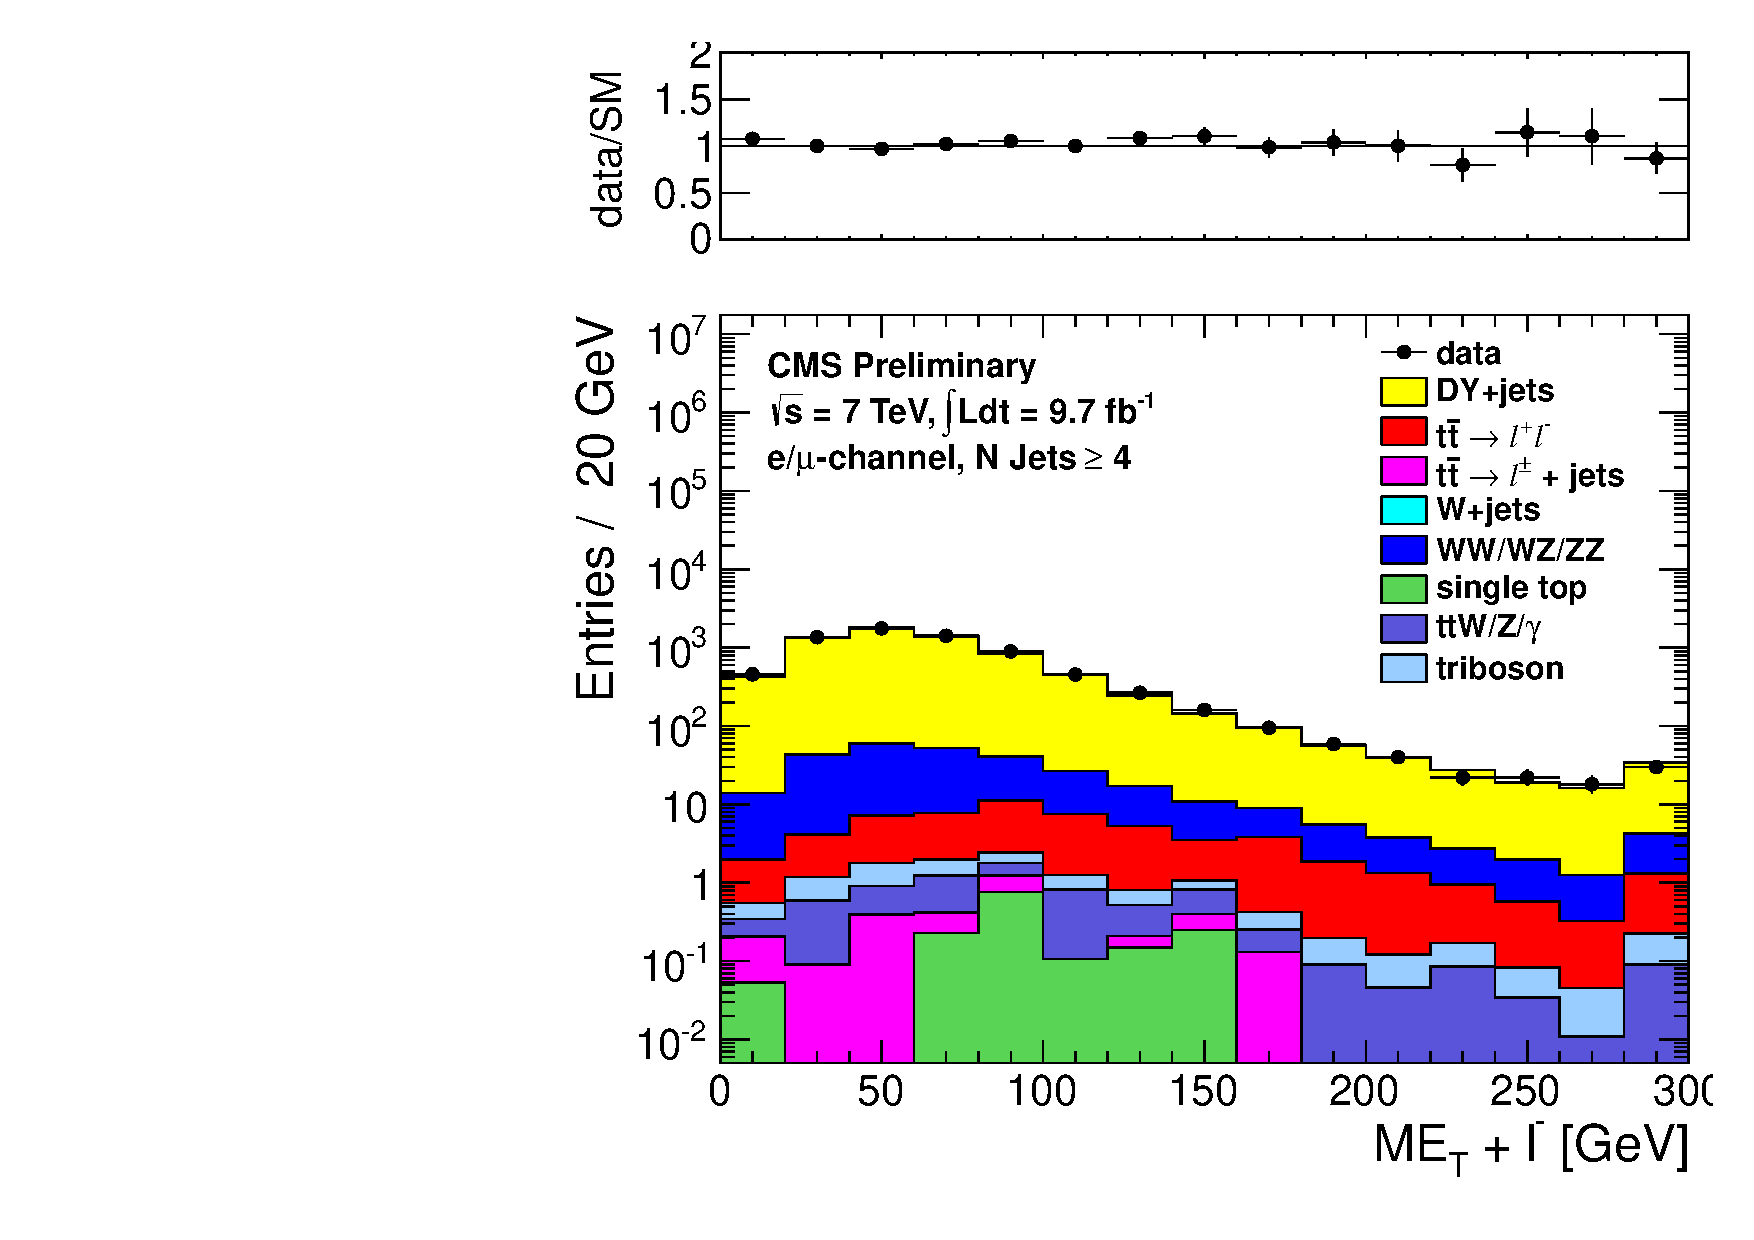
\includegraphics[width=0.5\linewidth]{plots/CR2plots/met_lepcor_scaled_nj4_emucomb.pdf}
	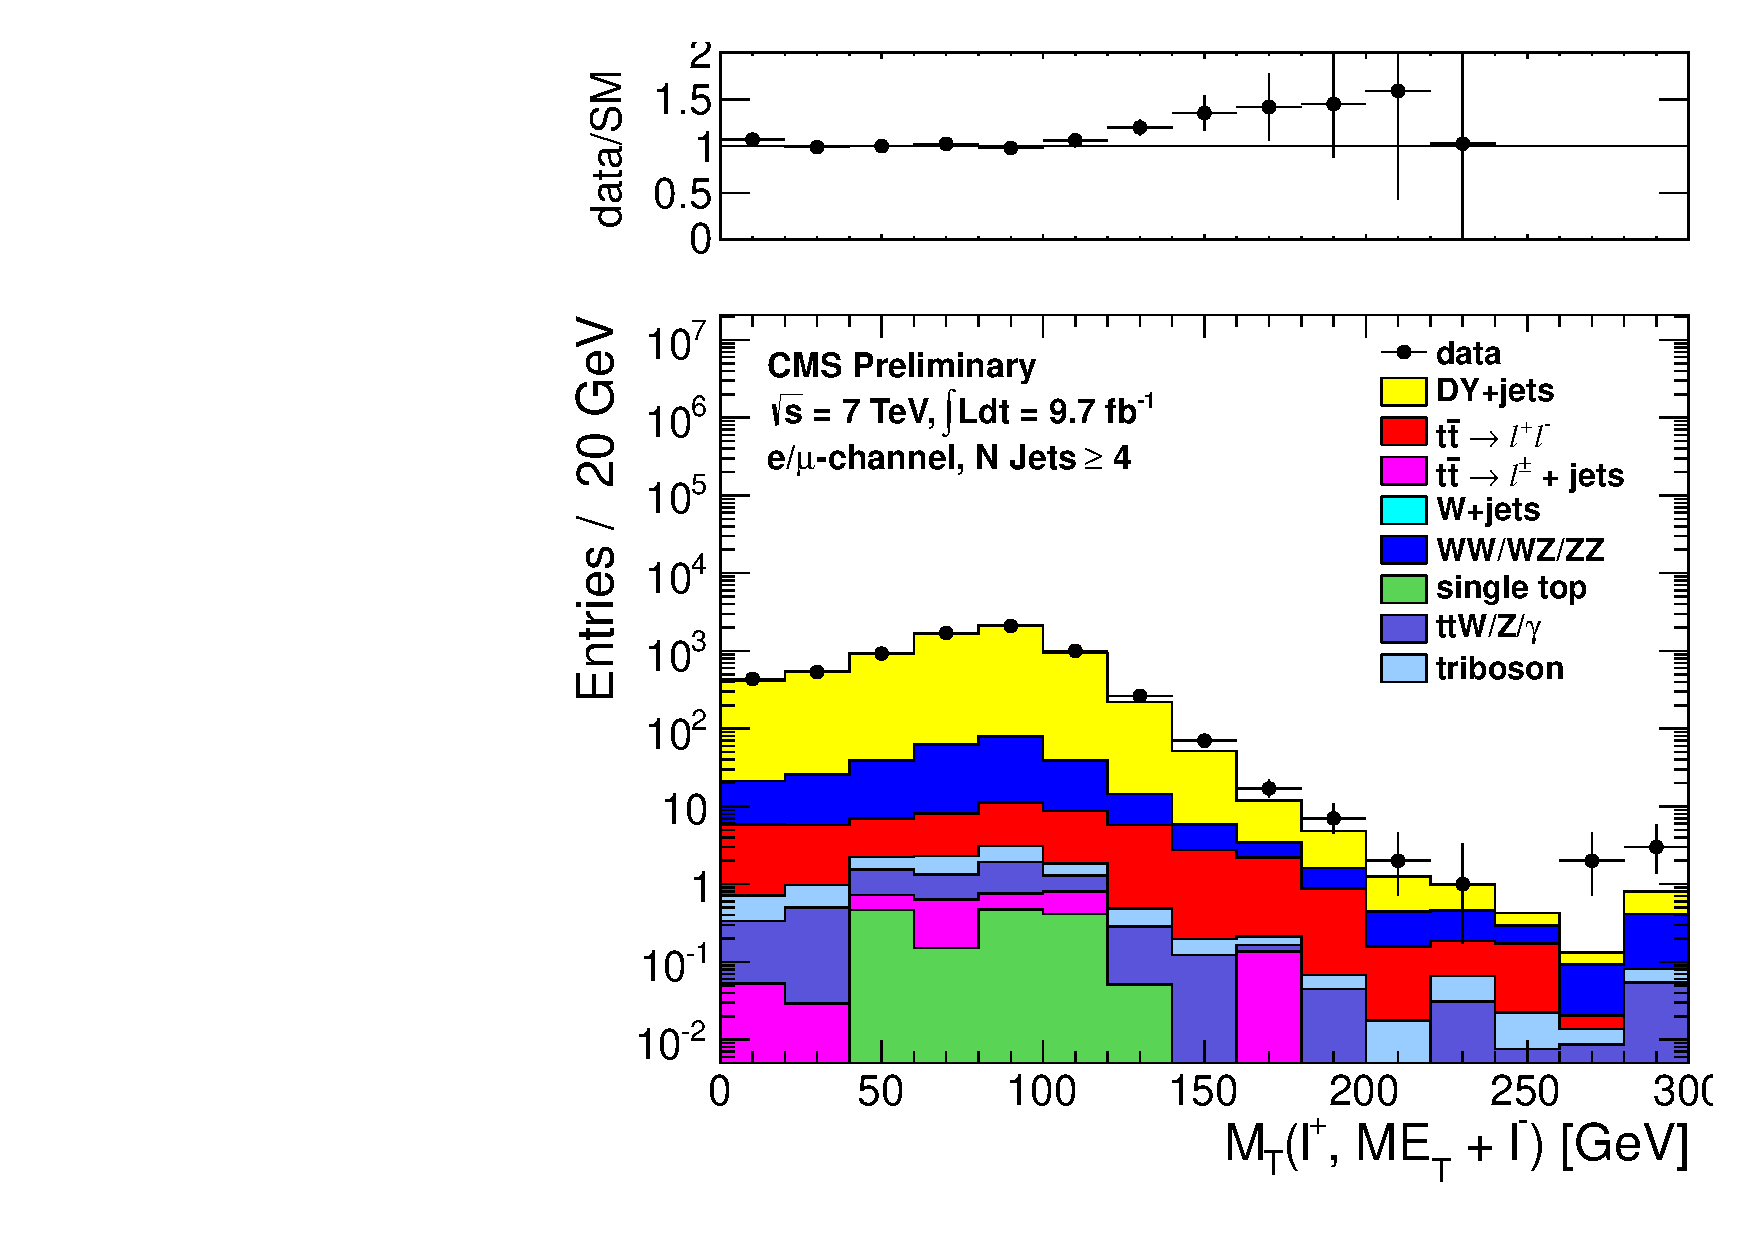
\includegraphics[width=0.5\linewidth]{plots/CR2plots/mt_lepcor_scaled_nj4_emucomb.pdf}%
	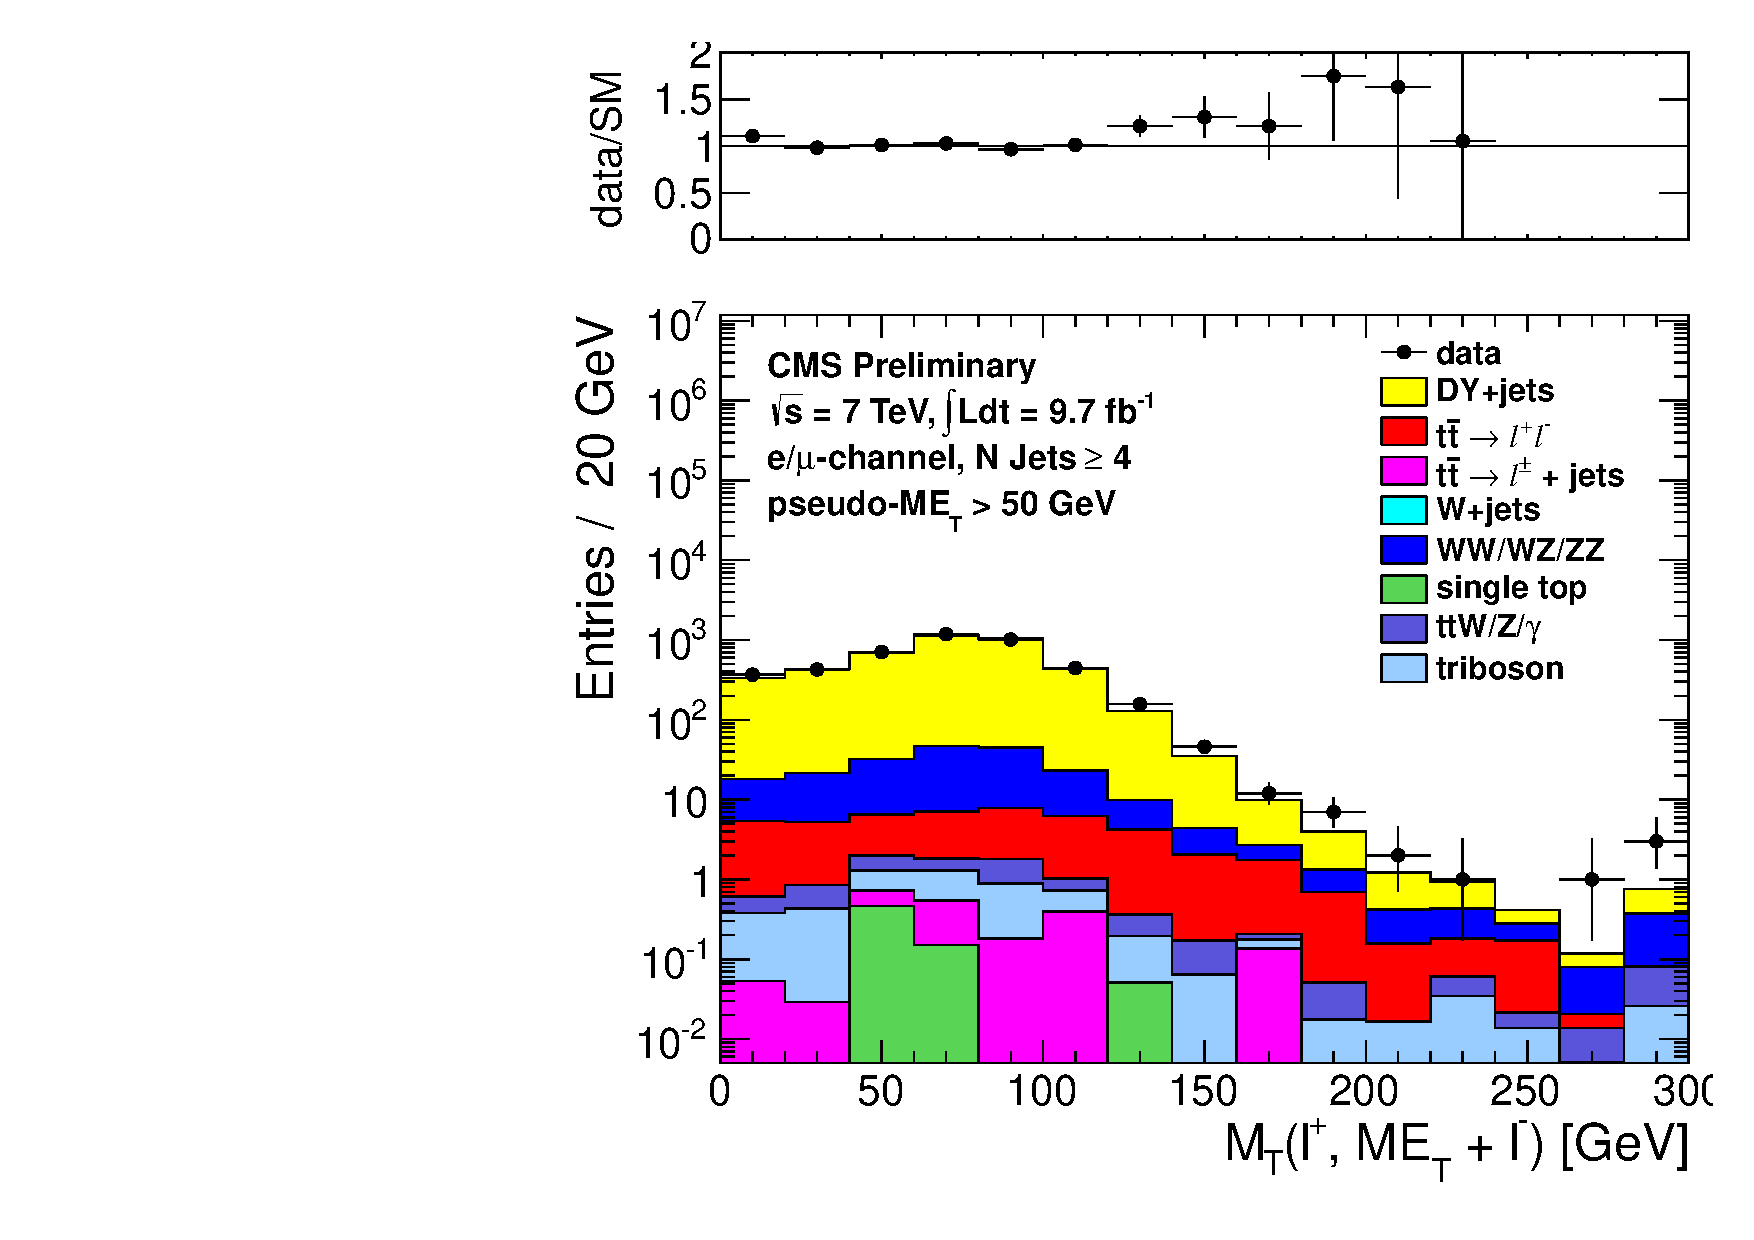
\includegraphics[width=0.5\linewidth]{plots/CR2plots/mt_lepcor_scaled_met50_nj4_emucomb.pdf}
    \caption{
      Comparison of the \met\ (top, left), pseudo-\met\ (top, right)
      and pseudo-\mt\ (bottom) distributions in data vs. MC for events
      satisfying the requirements of CR2, combining both the muon and
      electron channels. The pseudo-\mt\ distributions are shown
      before any additional requirements (bottom, left) and after
      requiring pseudo-\met>50 GeV (bottom, right).
\label{fig:cr2met} 
}  
      \end{center}
\end{figure}

\begin{figure}[hbt]
  \begin{center}
	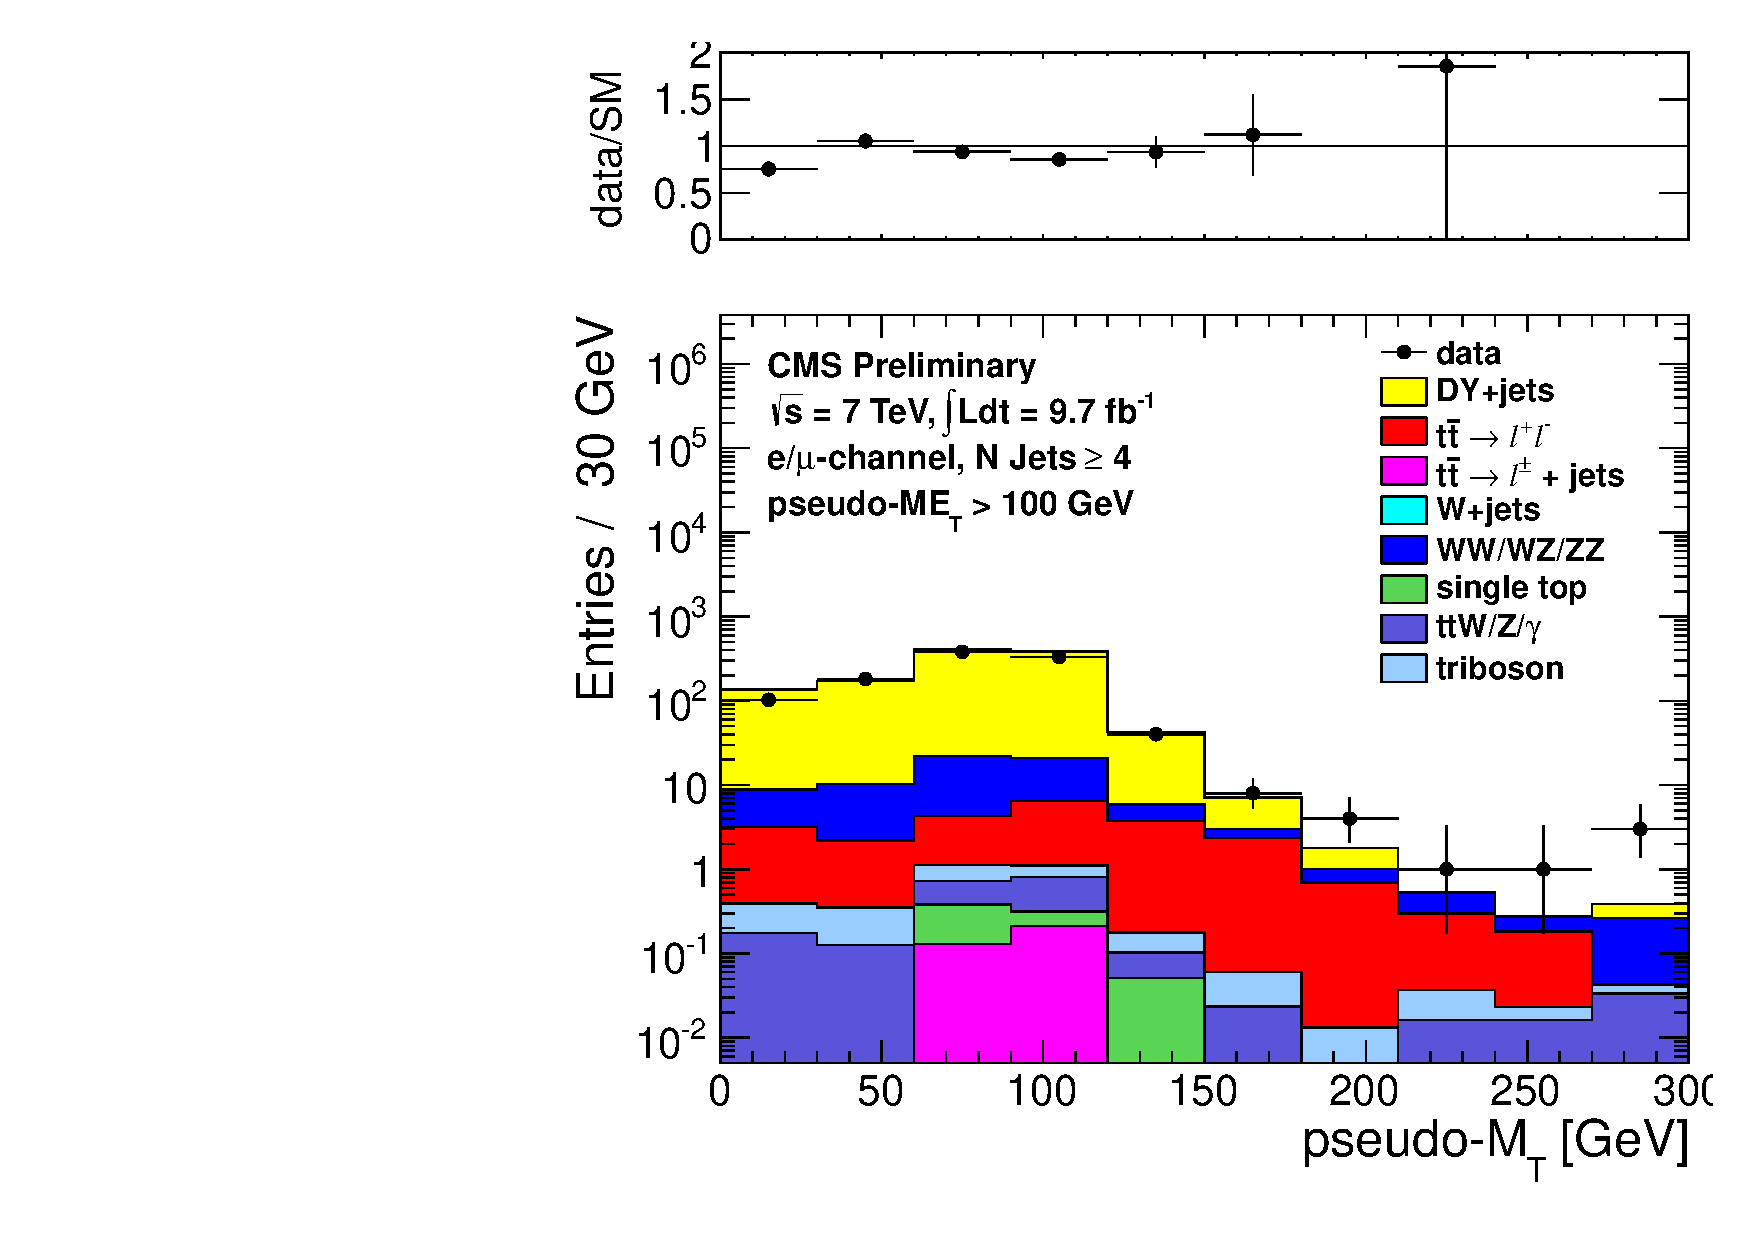
\includegraphics[width=0.5\linewidth]{plots/CR2plots/mt_lepcor_scaled_met100_nj4_emucomb.pdf}%
	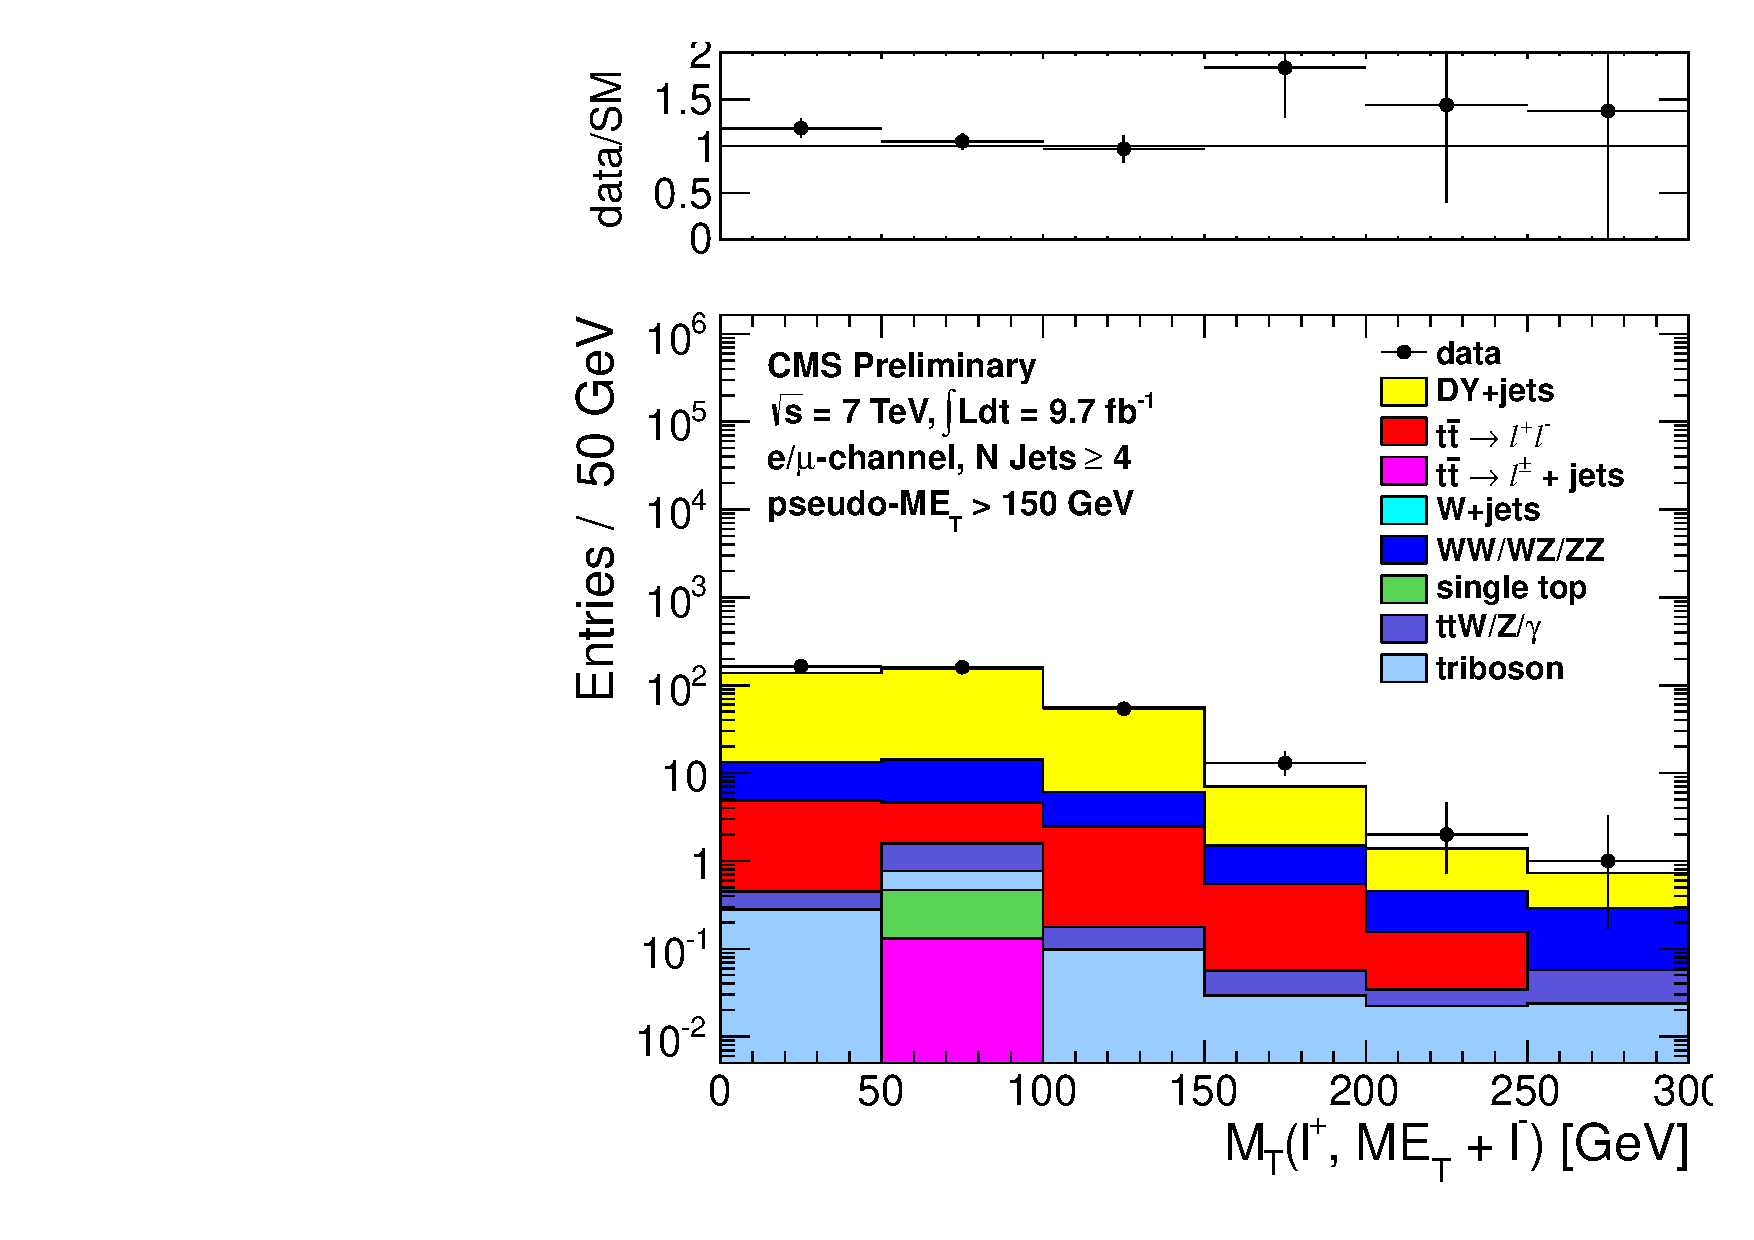
\includegraphics[width=0.5\linewidth]{plots/CR2plots/mt_lepcor_scaled_met150_nj4_emucomb.pdf}
	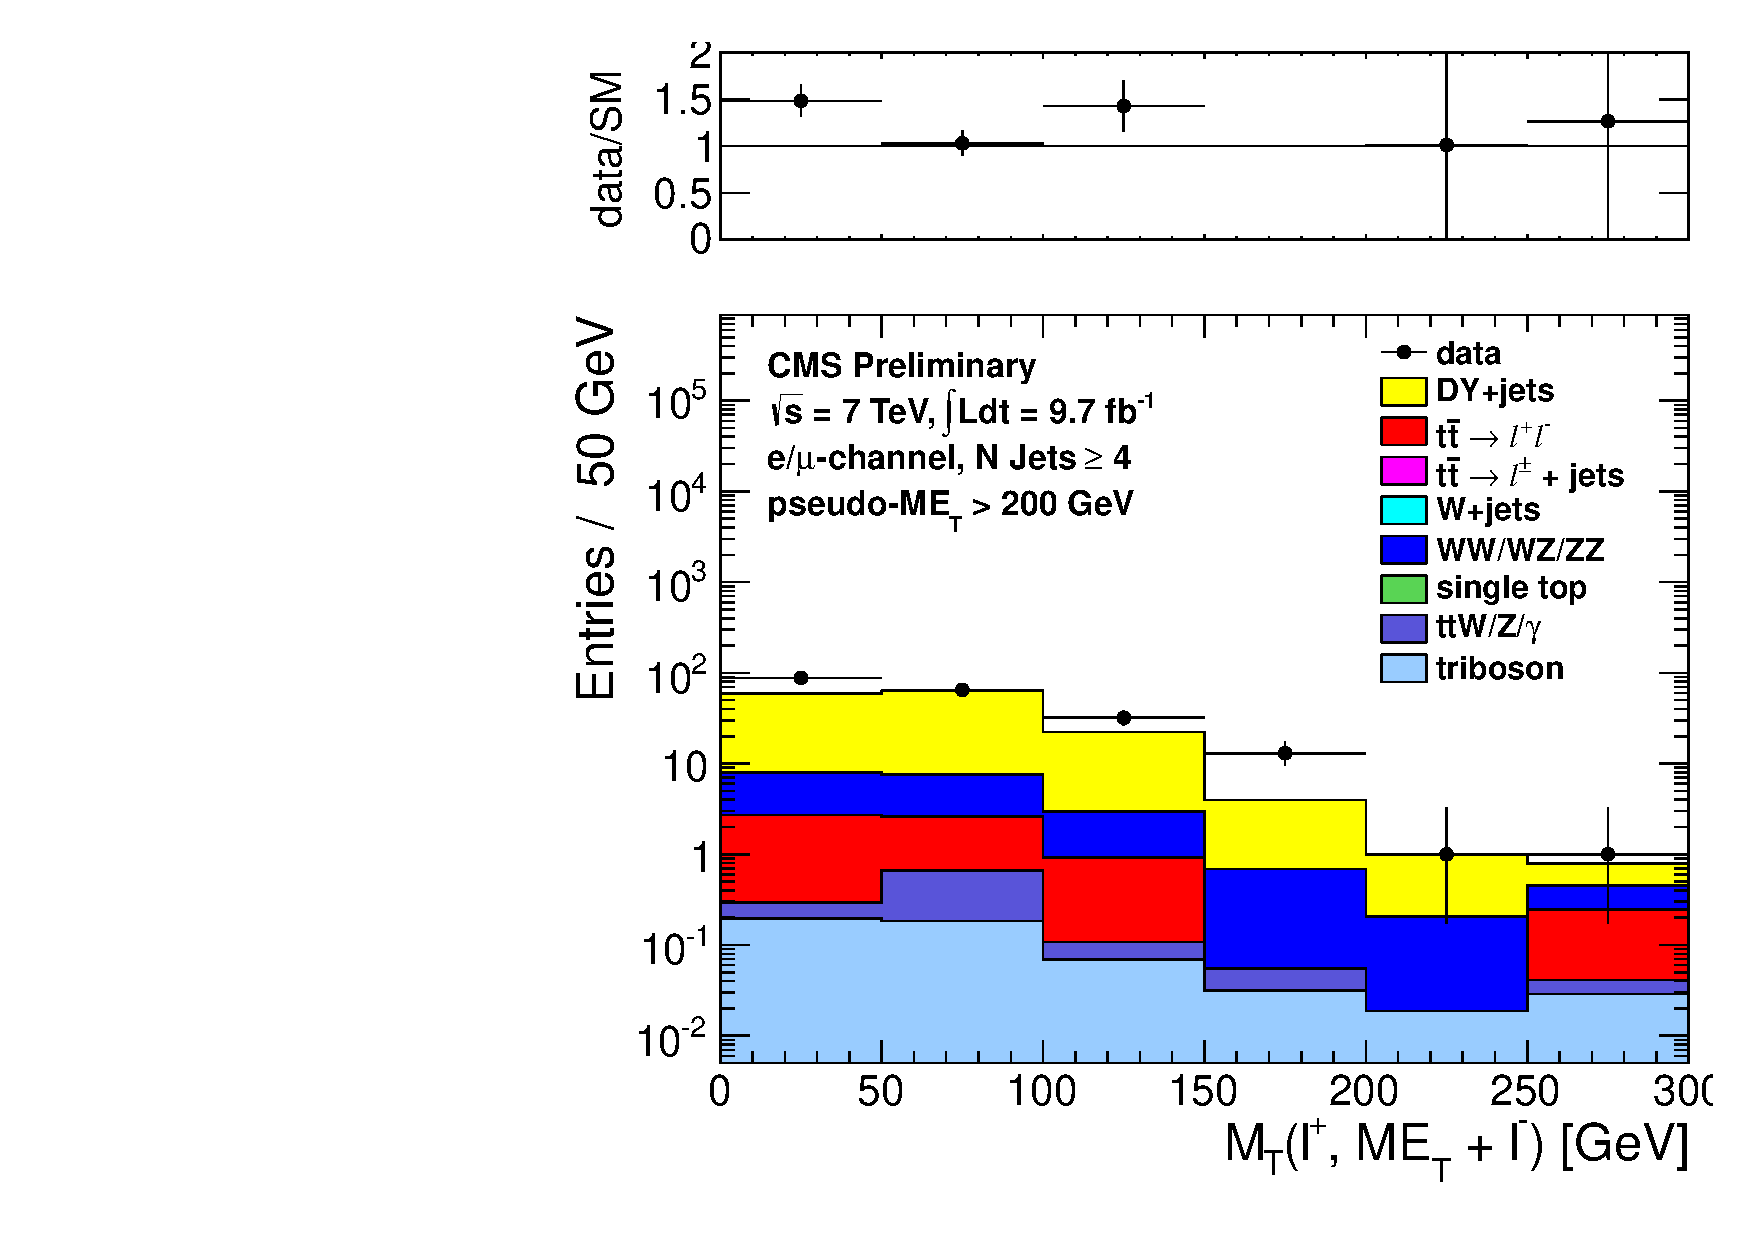
\includegraphics[width=0.5\linewidth]{plots/CR2plots/mt_lepcor_scaled_met200_nj4_emucomb.pdf}%
	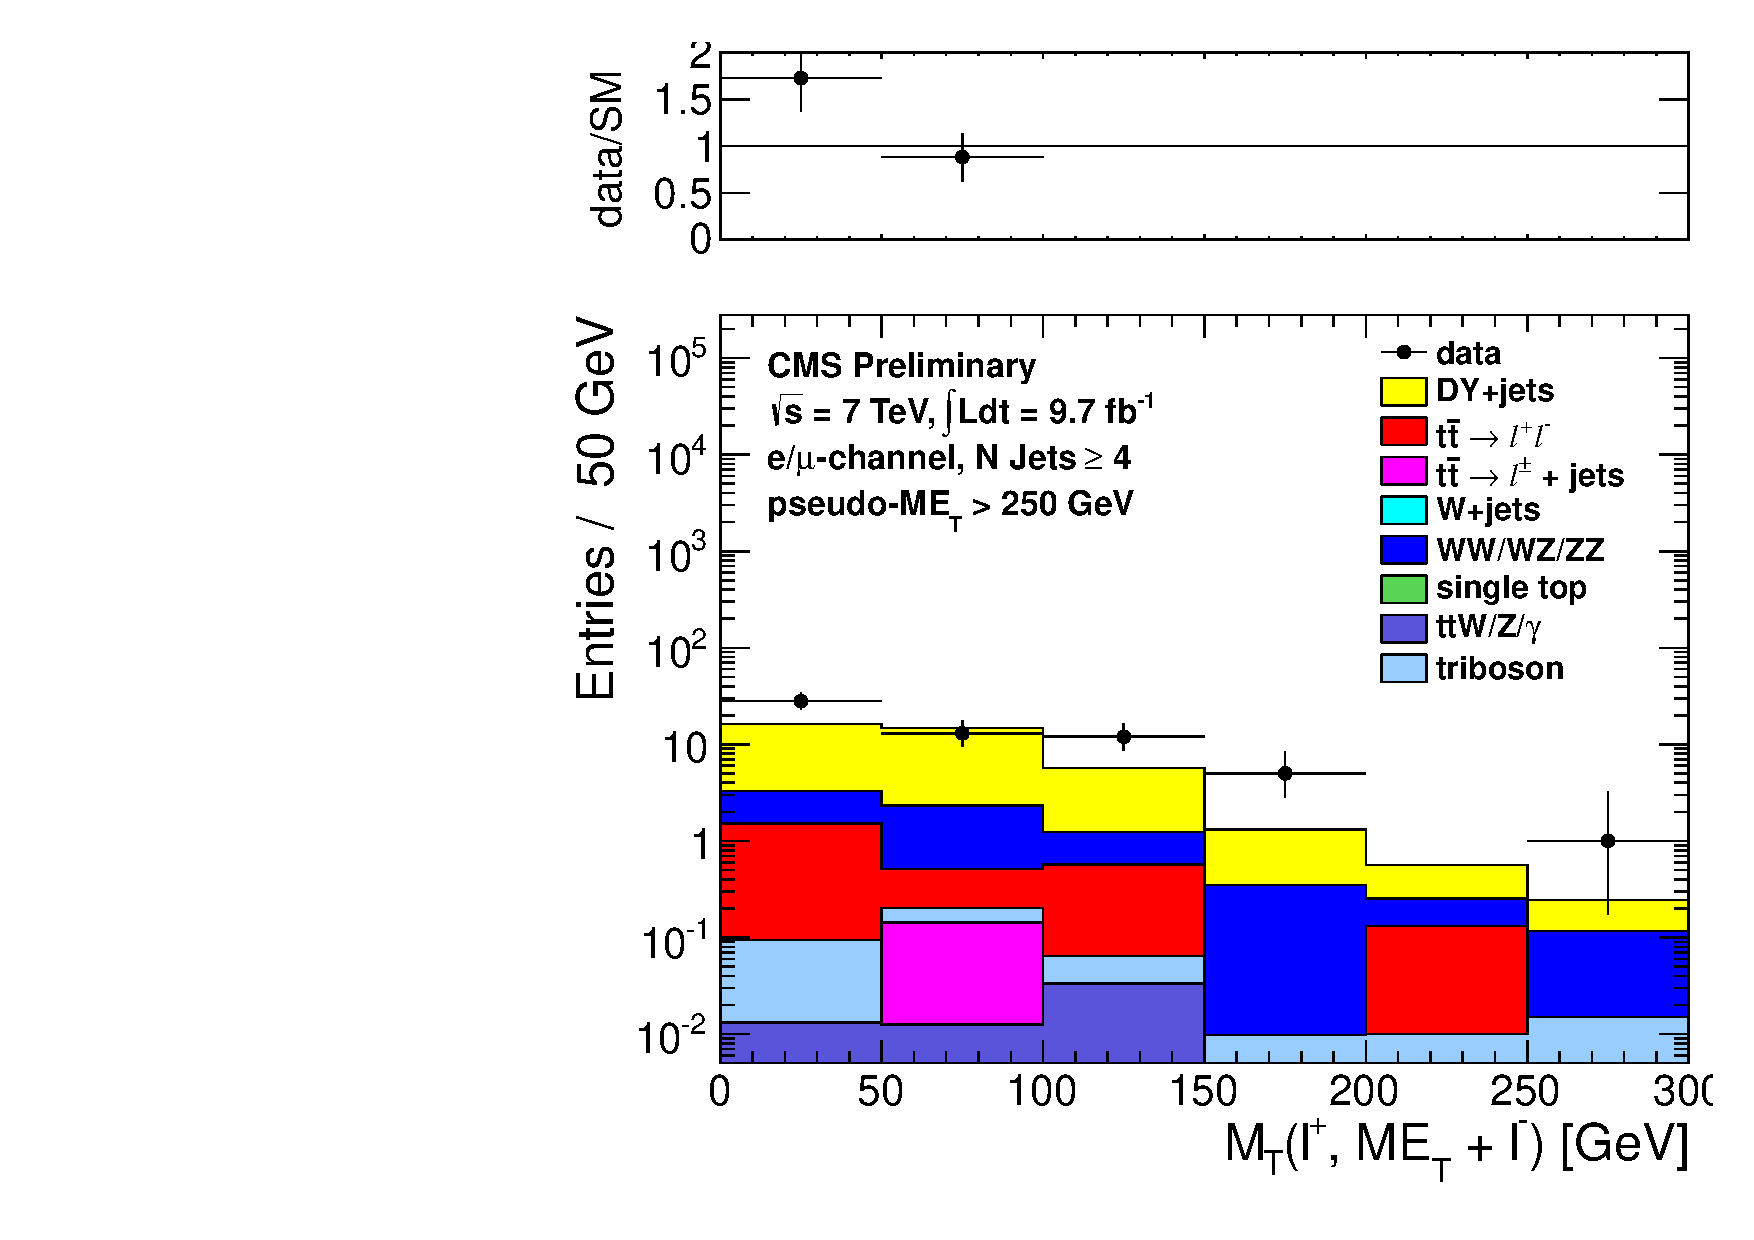
\includegraphics[width=0.5\linewidth]{plots/CR2plots/mt_lepcor_scaled_met250_nj4_emucomb.pdf}
    \caption{
      Comparison of the \mt\ distribution in data vs. MC for events
      satisfying the requirements of CR2, combining both the muon and
      electron channels. The pseudo-\met\ requirements used are
      100 GeV (top, left), 150 GeV (top, right), 200 GeV (bottom,
      left) and 250 GeV (bottom, right).
\label{fig:cr2mtrest} 
}  
      \end{center}
\end{figure}
\clearpage